
\subsection{\whatIsTitle: Overview}

%%%Insert this to get the typewriter font so it looks like a real movie script
{\ttfamily
\fontdimen2\font=0.4em
\fontdimen3\font=0.2em
\fontdimen4\font=0.1em
\fontdimen7\font=0.1em
\hyphenchar\font=`\-


%%%%put a hypertarget around the opening bit of text
\hypertarget{video_what_is_overview}{In this course, we start with linear systems} 
\begin{equation}\label{linsys}
\left\{
\begin{array}{ccc}
f_1(x_1,\ldots,x_m)& = &a_1\\[1mm]
\vdots&&\vdots\\[1mm]
f_n(x_1,\ldots,x_m) &=& a_n\, ,
\end{array}
\right.
\end{equation}
and discuss how to solve them.

We end with the problem of finding a least squares fit---find the line that best fits a given data set:
\begin{center}
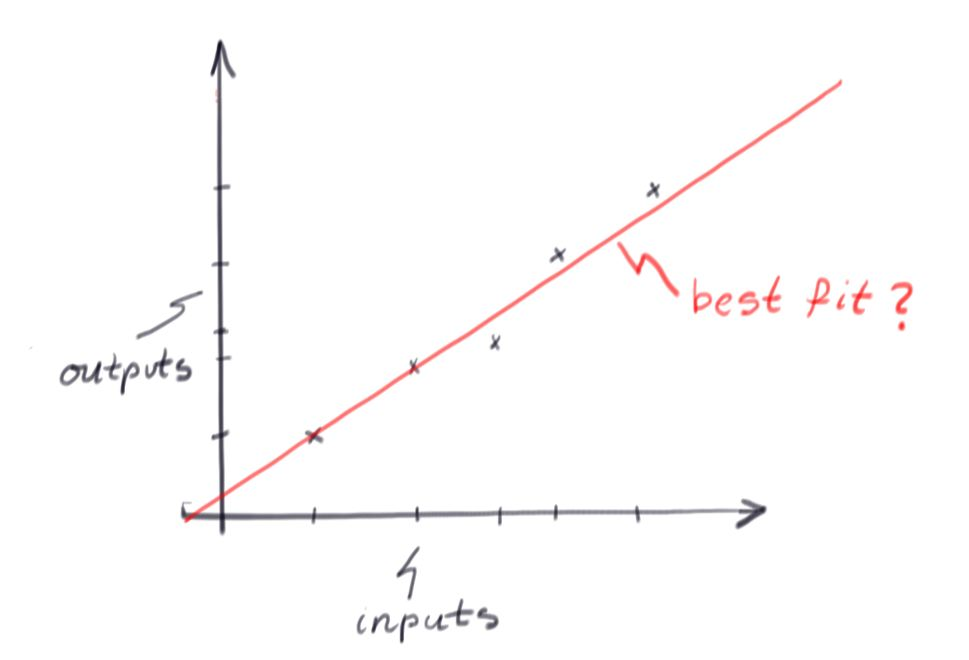
\includegraphics[scale=.2]{best_fit.jpg}
\end{center}

In equation~\eqref{linsys} we have $n$ {\it linear} functions called $f_1,\ldots, f_n$, $m$ un\-knowns $x_1,\ldots, x_m$
and $n$ given constants $a_1,\ldots,a_n$. We need to say what it means for a function to be linear.
A linear function has the {\it additive property}
$$
f(a+b)=f(a)+f(b)\, .
$$
The solution to this is
$$
f(x)=\lambda x\, ,
$$
for some constant $\lambda$. The plot of this is just a straight line through the origin with 
slope~$\lambda$
\begin{center}
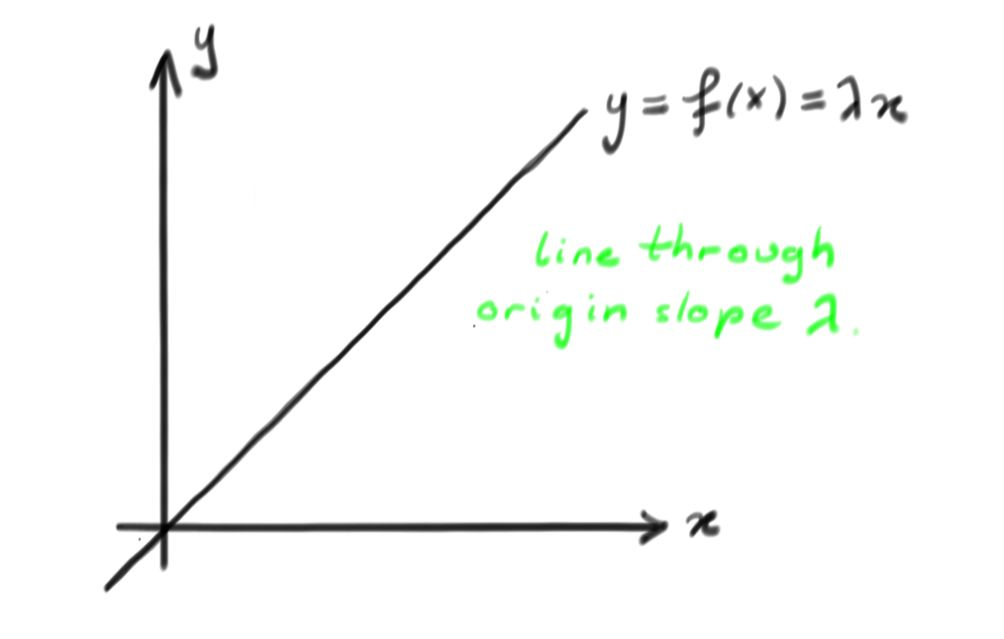
\includegraphics[scale=.2]{line_through_origin.jpg}
\end{center}

We should also check that our solution obeys the linearity property. The logic is to start with the left hand side $f(a+b)$
and try to turn it into the right hand side $f(a)+f(b)$ using correct manipulations:
$$
f(a+b)=\lambda(a+b) =\lambda a + \lambda b = f(a) + f(b)\, .
$$
The first step here just plugs $a+b$ into $f(x)$, the second is the distributive property, and in the third we recognize that $\lambda a = f(a)$ and $\lambda b = f(b)$.
This proves our claim.

For functions of many variables, linearity must hold for every slot. For a linear function of two variables $f(x,y)$ this means
$$
f(a+b,c+d)=f(a,c)+f(b,d)\, .
$$

We finish with a question. The plot of $f(x)=\lambda x + \beta$ is a straight line, but does it obey the linearity property?

%%%%don't forget to close the bracket so the stuff after your file doesn't look like a movie!
}

\newpage
